\newcommand{\ClassPath}{../VIU_TFM_LaTeX_template}
\documentclass{\ClassPath/viu-tfm-template}
\usepackage{multicol}

\definecolor{maincolor}{HTML}{f25416}

%--------------------------------------------------------------------------
% Definiciones necesarias Modifica con tus datos
%--------------------------------------------------------------------------
\def\nombre{Gómez Olivencia, Rubén}
\def\dni{78910013-A}
\def\titulo{Despliegue de aplicaciones en AWS}
\def\subtitulo{(Beanstalk, Automatización con Gitlab y Terraform)}
\def\titulacion{Máster Universitario en Desarrollo de Aplicaciones y Servicios Web}
\def\curso{2022-2023}

%Los siguientes son opcionales: si no se ponen, la portada cambia un poco. Ideal para escribir artículos/trabajos cortos
\def\dirige{}
\def\codirige{}
\def\convocatoria{}
\def\asignatura{Computación en la nube}


% importar fichero de Bibliografía
%\addbibresource{Actividad_1.bib}

\begin{document}
    \graphicspath{{../VIU_TFM_LaTeX_template/}}

    \coverpage

    \tableofcontents

\chapter{Introducción}

A la hora de poner un proyecto en producción era habitual realizar el despliegue de manera manual, teniendo que realizar la instalación y la configuración de cada servicio que se vaya a necesitar.

A día de hoy el despliegue manual ha sufrido muchas mejoras gracias a los sistemas de contenedores, como ejemplo \href{https://www.docker.com/}{Docker} o sistemas PaaS (plataformas como servicio) como \href{https://en.wikipedia.org/wiki/AWS_Elastic_Beanstalk}{AWS Elastic Beanstalk}.

Por otro lado, tenemos la posibilidad de realizar despliegues automatizados gracias a los nuevos sistemas de integración continua y despliegue continuo (CI/CD), muy utilizado en la metodología DevOps. De esta manera, una vez creado el \textit{pipeline} de ejecución, el despliegue siempre se realizará de igual manera.

Si al punto anterior le añadimos la creación de toda la infraestructura mediante código (IaC, \textit{Infraestructure as code}), pasar de un proveedor de servicios en nube a otro será mucho más sencillo.

En este documento usaremos la aplicación \href{https://flarum.org/}{Flarum} como ejemplo para realizar los distintos despliegues explicados previamente.


\chapter{Base de datos RDS}
Para la aplicación se va a necesitar una base de datos, por lo que va a ser lo primero que se va a desplegar.

AWS permite realizar el despliegue de distintos gestores de bases de datos a través de su servicio \textbf{RDS} (\textit{Relational Database Service}). En este caso se va a desplegar un RDS de MySQL 5.X con las siguientes características:

\begin{itemize}
    \item RDS de tipo db.t3.micro
    \item Almacenamiento 20Gib SSD de uso general (gp2).
    \item Cifrado en reposo habilitado.
    \item Nombre bd = DB\_flarum
    \item User = admFlarum
    \item Password = Viu2022Flarum
    \item Charset = utf8mb4
    \item Collation = utf8mb4\_unicode\_ci
\end{itemize}

Es importante añadirle un grupo de seguridad que permita todo el tráfico entrante procedente de la red del VPC de AWS (por defecto 172.31.0.0/16).


\begin{center}
    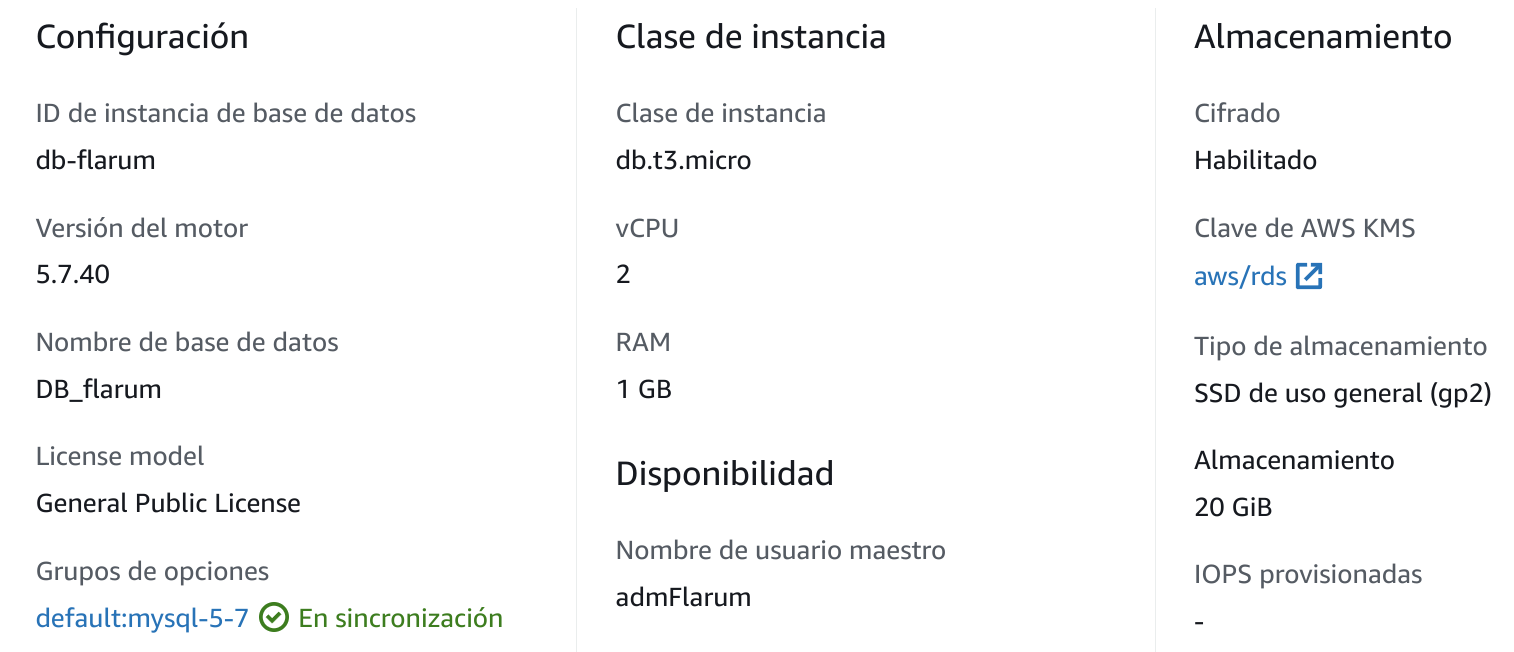
\includegraphics[frame,width=0.8\linewidth]{img/rds.png}
\end{center}

Con esto ya tendríamos creada la base de datos.


\chapter{Despliegue con AWS Elastic Beanstalk}

\href{https://aws.amazon.com/es/elasticbeanstalk/}{Amazon Elastic Beanstalk} nos permite crear y desplegar aplicaciones web de manera sencilla sin tener que depender de la tediosa configuración que hay detrás de ello.

Para realizar el despliegue de Flarum se han utilizado la siguiente configuración personalizada, a través del editor avanzado al crear el entorno de Beanstalk:
\vspace{-15pt}
\begin{itemize}
    \item \textbf{Nombre de la aplicación} = flarum
    \item \textbf{Nombre del entorno} = pro-XXYY-08masw
    \item Sin balanceador de carga.
    \item \textbf{Entorno}: PHP 8.0
    \item \textbf{Servidor Web} = apache
    \item \textbf{Raíz del documento}: /public
    \item \textbf{Mostrar errores}: On
    \item \textbf{Código fuente} de la aplicación obtenido de \href{https://amn-viu-resources-public.s3.eu-west-1.amazonaws.com/08masw/actividad2/flarum_php8.0.zip}{aquí}.
\end{itemize}

Tras crear el entorno, nos aparecerá a modo resumen en el interfaz lo siguiente:
\begin{center}
    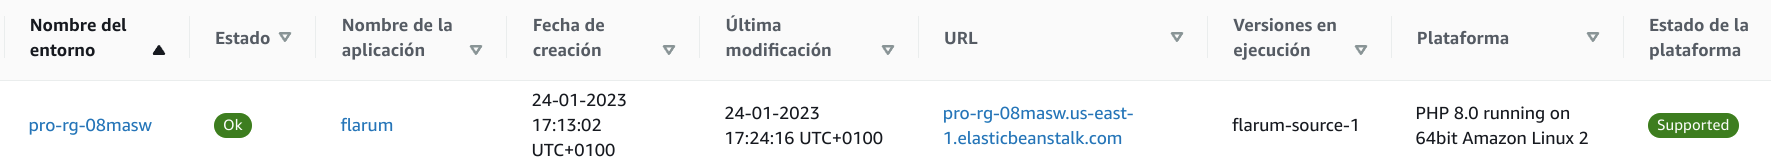
\includegraphics[frame,width=\linewidth]{img/beanstalk.png}
\end{center}

Para poder acceder al nuevo entorno a través del navegador web, vemos cómo se nos ha creado una URL propia \href{http://pro-rg-08masw.us-east-1.elasticbeanstalk.com/}{pro-rg-08masw.us-east-1.elasticbeanstalk.com}, que al acceder nos muestra el panel de configuración de Flarum:

\vspace{-10pt}
\begin{center}
    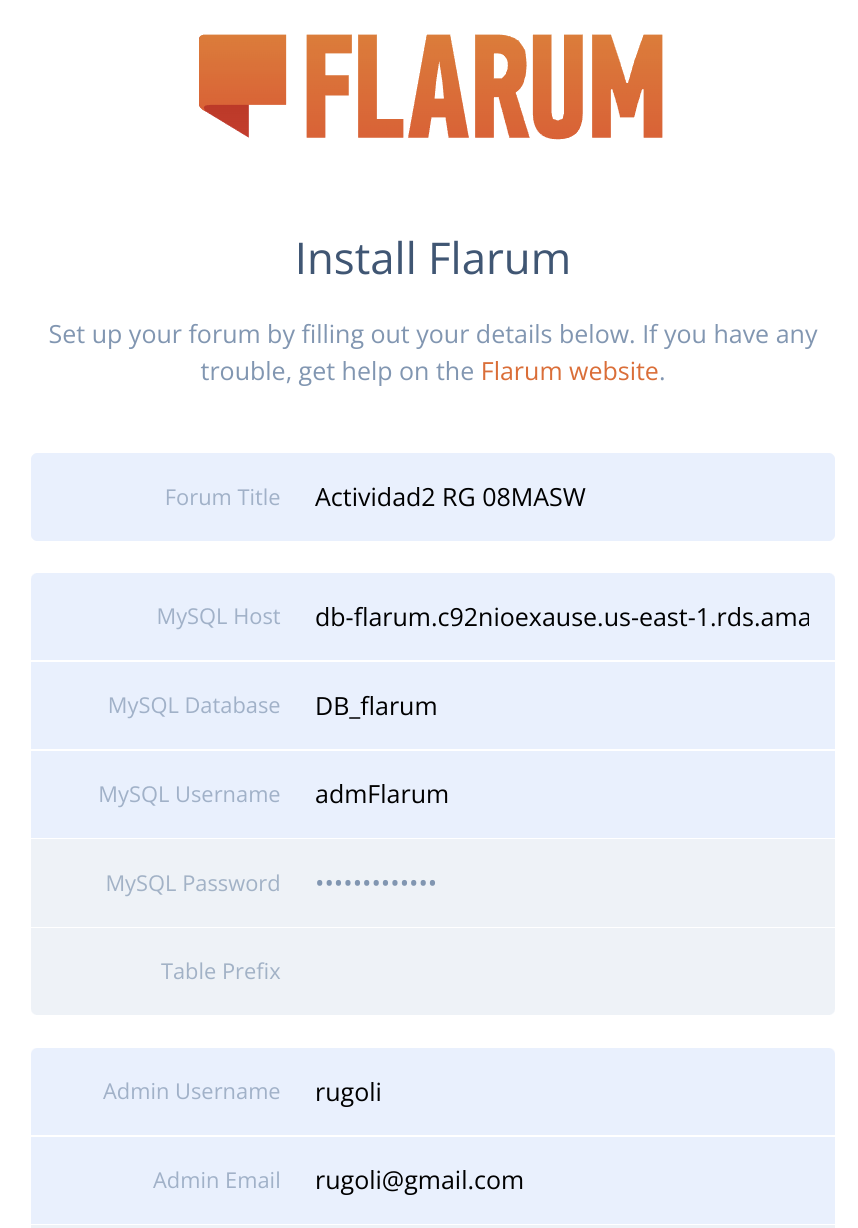
\includegraphics[frame,width=0.63\linewidth]{img/flarum-0.png}
\end{center}

En este formulario nos aparecen las opciones que debemos rellenar para que se acceda a la base de datos creada previamente. Tras introducir los datos de manera correcta, la aplicación desplegará las tablas que necesita y ya podremos acceder a la aplicación.

\begin{center}
    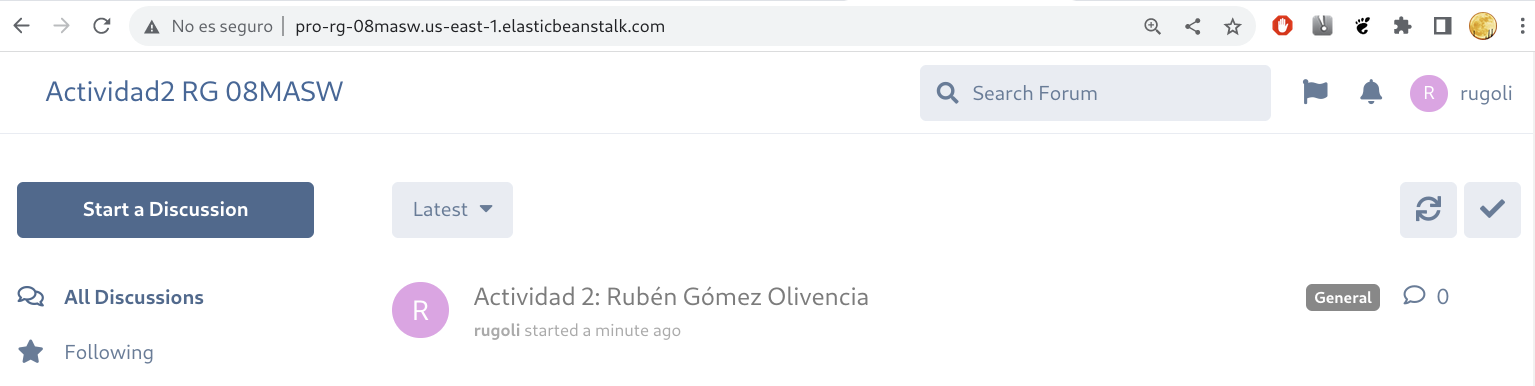
\includegraphics[frame,width=\linewidth]{img/flarum-1.png}
\end{center}

En la imagen anterior se puede cómo se ha podido crear una nueva entrada en el foro recién desplegado.


\chapter{Despliegue automatizado desde GitLab}

Para este apartado vamos a utilizar \href{https://gitlab.com/}{GitLab} para realizar el despliegue de manera automatizada a través de su sistema de integración continua y despliegue continuo (CI/CD).

Lo primero que tenemos que hacer es crear un nuevo repositorio con el código obtenido de este \href{https://amn-viu-resources-public.s3.eu-west-1.amazonaws.com/08masw/actividad2/flarum_php8.0.zip}{enlace}.

\begin{center}
    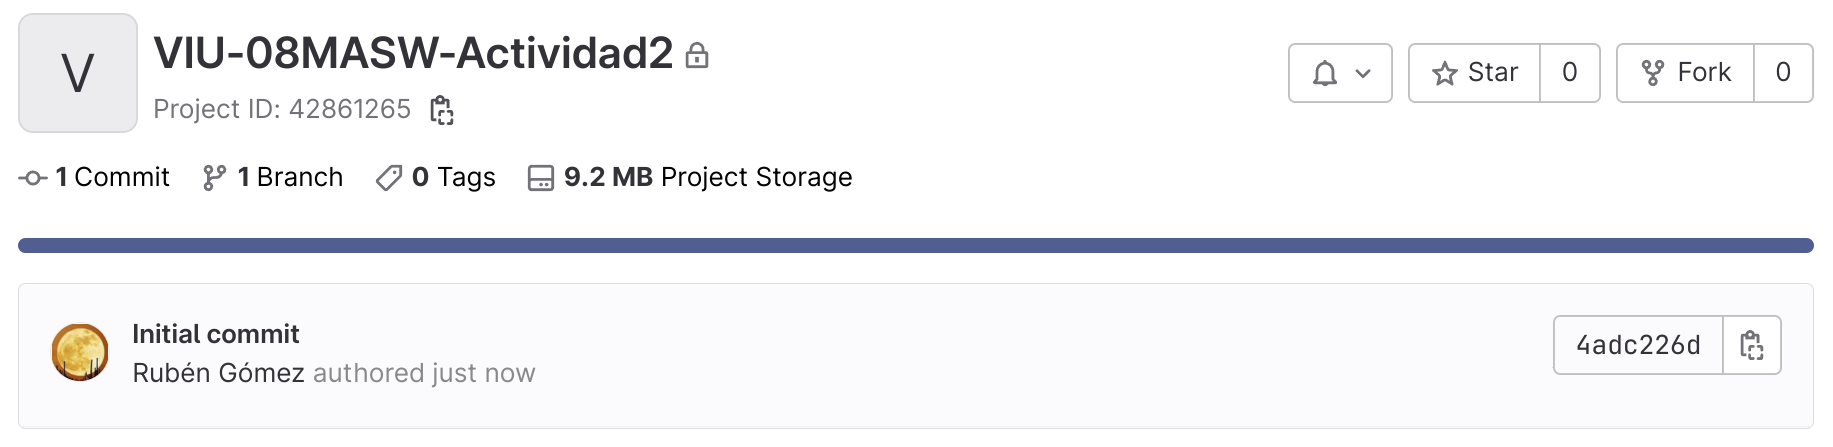
\includegraphics[frame,width=\linewidth]{img/gitlab.png}
\end{center}

Tras subir el código hay que realizar las siguientes modificaciones:

\begin{itemize}
    \item Añadir el fichero \configfile{.gitlab-ci.yml}. Es el encargado de lanzar el \textit{pipeline}, que son las instrucciones para realizar el despliegue automatizado que ejecuta GitLab al recibir un commit del código.
\end{itemize}
\begin{mycode}{Parte del .gitlab-ci.yml}{yaml}{{\scriptsize }}
image: "php:8.0"
stages:
  - build
  - deploy
cache:
  key: cache-key
  paths:
  - vendor/
  - node_modules/
before_script:
  - apt-get update
  - apt-get install -y python3 python3-pip wget zip unzip git
  - pip -V
.build:
  script:
    - echo "Building app"
    - apt-get install -y libpng-dev libxml2-dev libzip-dev sudo nodejs npm
    - wget https://composer.github.io/installer.sig -O - -q | tr -d '\n' > installer.sig
    - php -r "copy('https://getcomposer.org/installer', 'composer-setup.php');"
    - php composer-setup.php --install-dir=/usr/local/bin -filename=composer --version=2.0.14
    - php -r "unlink('composer-setup.php'); unlink('installer.sig');"
    # Extra PHP libraries
    - docker-php-ext-install gd
    - docker-php-ext-install soap
    - docker-php-ext-install zip
    - zip ../myapp.zip -r * .[^.]* >/dev/null
    - mv ../myapp.zip .
  artifacts:
    paths:
    - myapp.zip
    expire_in: 1 week\end{mycode}

\begin{itemize}
    \item Modificar el fichero \configfile{.elasticbeanstalk/config.pro.yml} para que el \textit{pipeline} anterior lo utilice para realizar el despliegue. El despliegue se realizará sobre el mismo Beanstalk creado previamente.

    \begin{mycode}{Fichero de configuración para Beanstalk}{yaml}{}
global:
  application_name: flarum
  default_ec2_keyname: null
  default_region: us-east-1
  include_git_submodules: true
  instance_profile: null
  platform_name: null
  platform_version: null
  profile: eb-cli
  sc: git
  workspace_type: Application
deploy:
  artifact: ./myapp.zip\end{mycode}

    \item Añadir \textbf{variables} de entorno dentro de GitLab. El valor de estas variables será sustituido dentro del pipeline. De esta manera no introducimos credenciales en el código fuente del repositorio.
    \begin{center}
        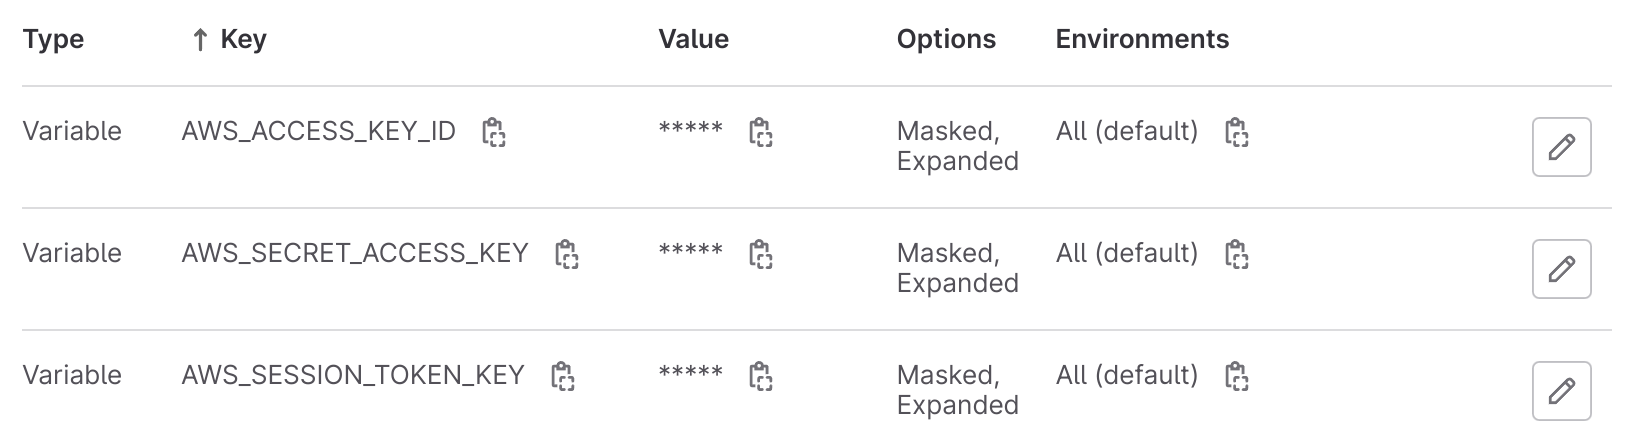
\includegraphics[frame,width=\linewidth]{img/gitlab-vars.png}
    \end{center}
\end{itemize}

Una vez realizadas las modificaciones, el \textit{pipeline} se ejecutará, y tras esperar a que termine los dos pasos del despliegue, en GitLab veremos un resumen:

\begin{center}
    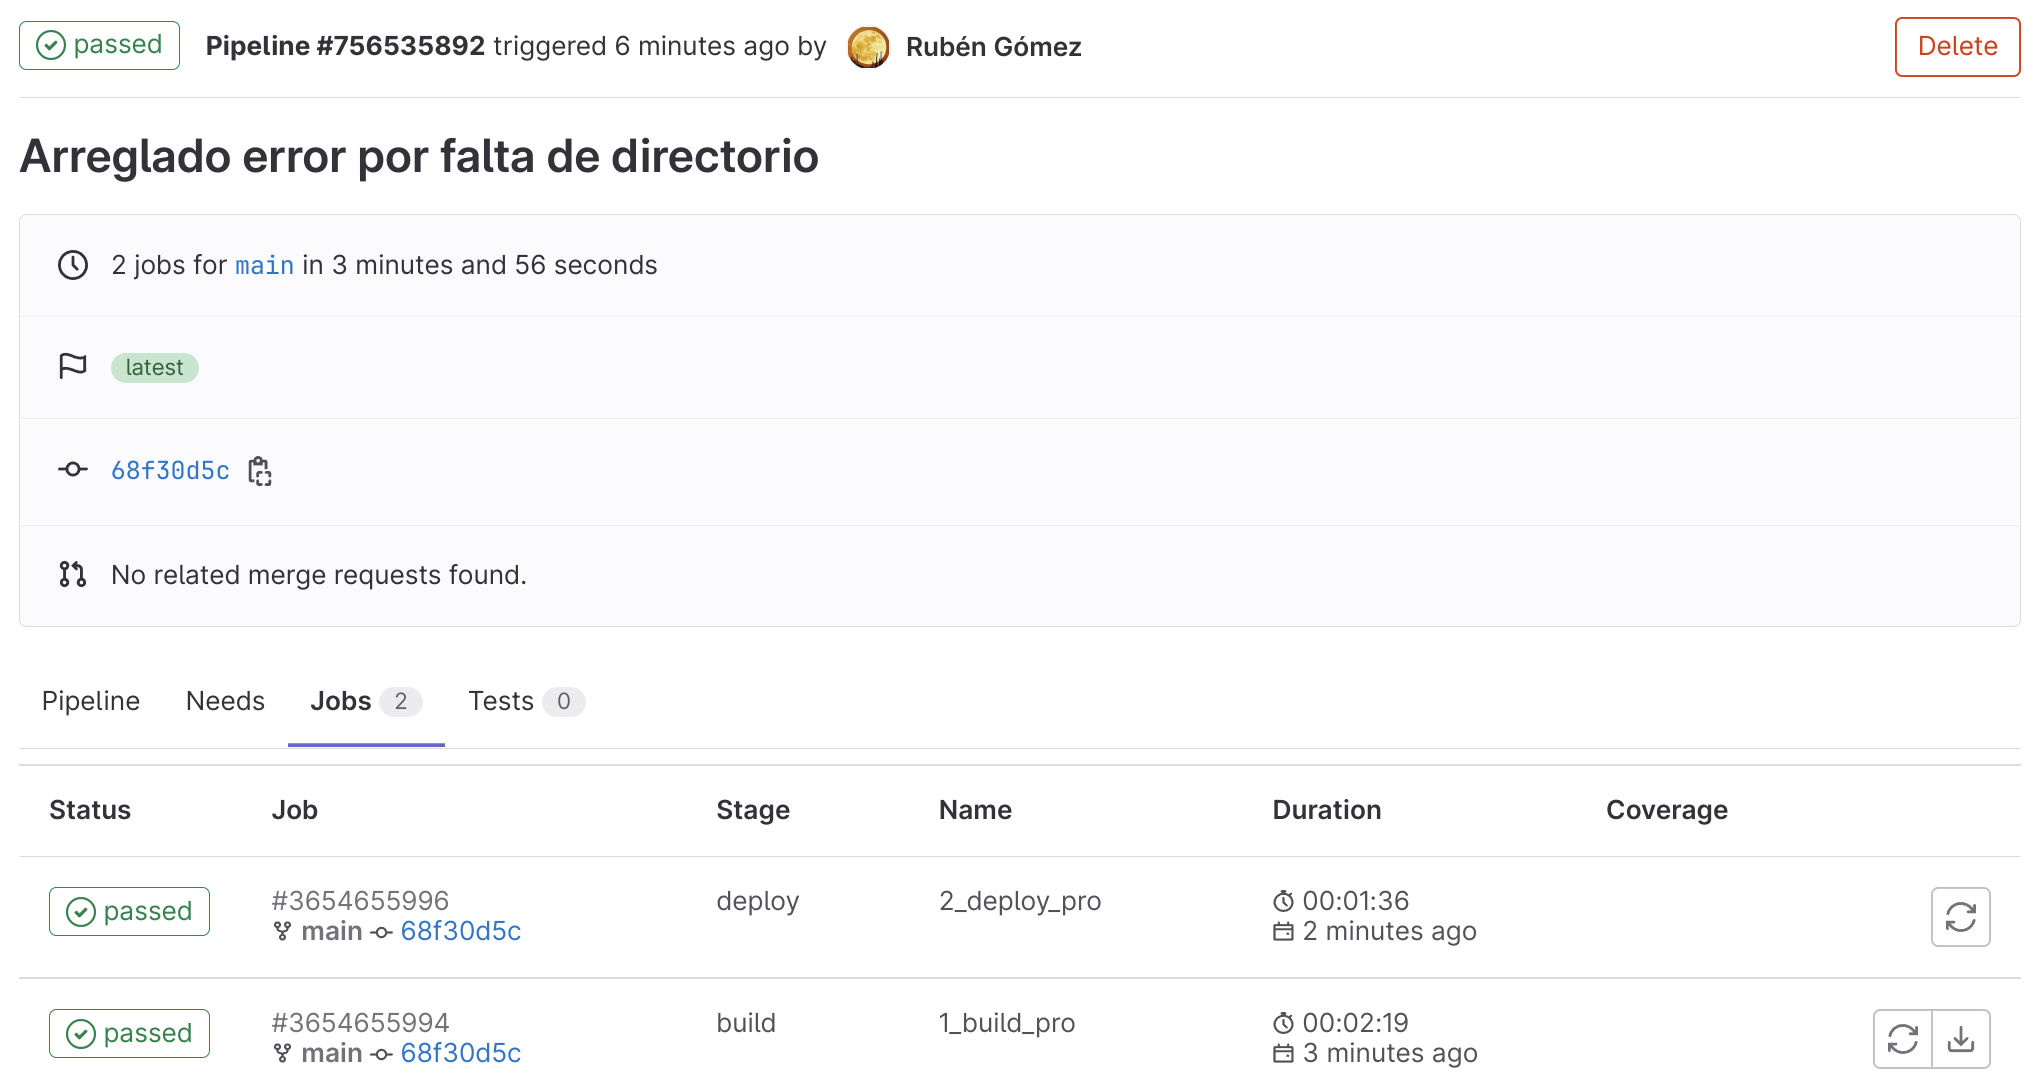
\includegraphics[frame,width=\linewidth]{img/gitlab-pipeline.png}
\end{center}

\begin{center}
    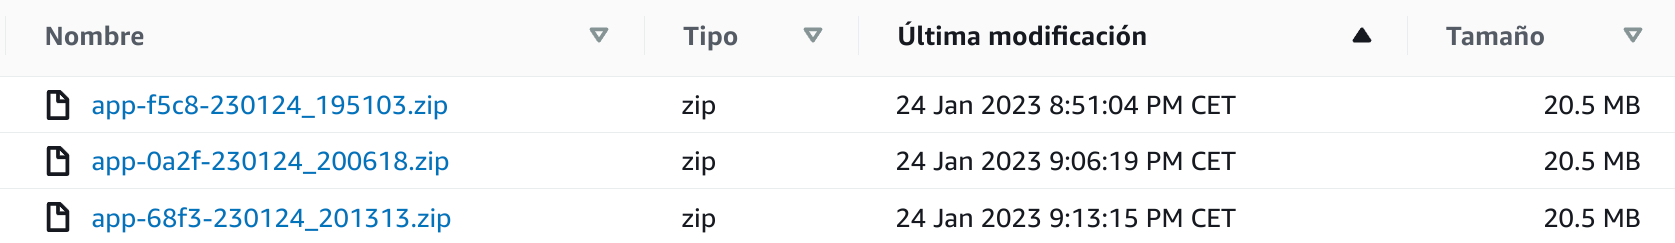
\includegraphics[frame,width=\linewidth]{img/s3.png}
\end{center}



\begin{center}
    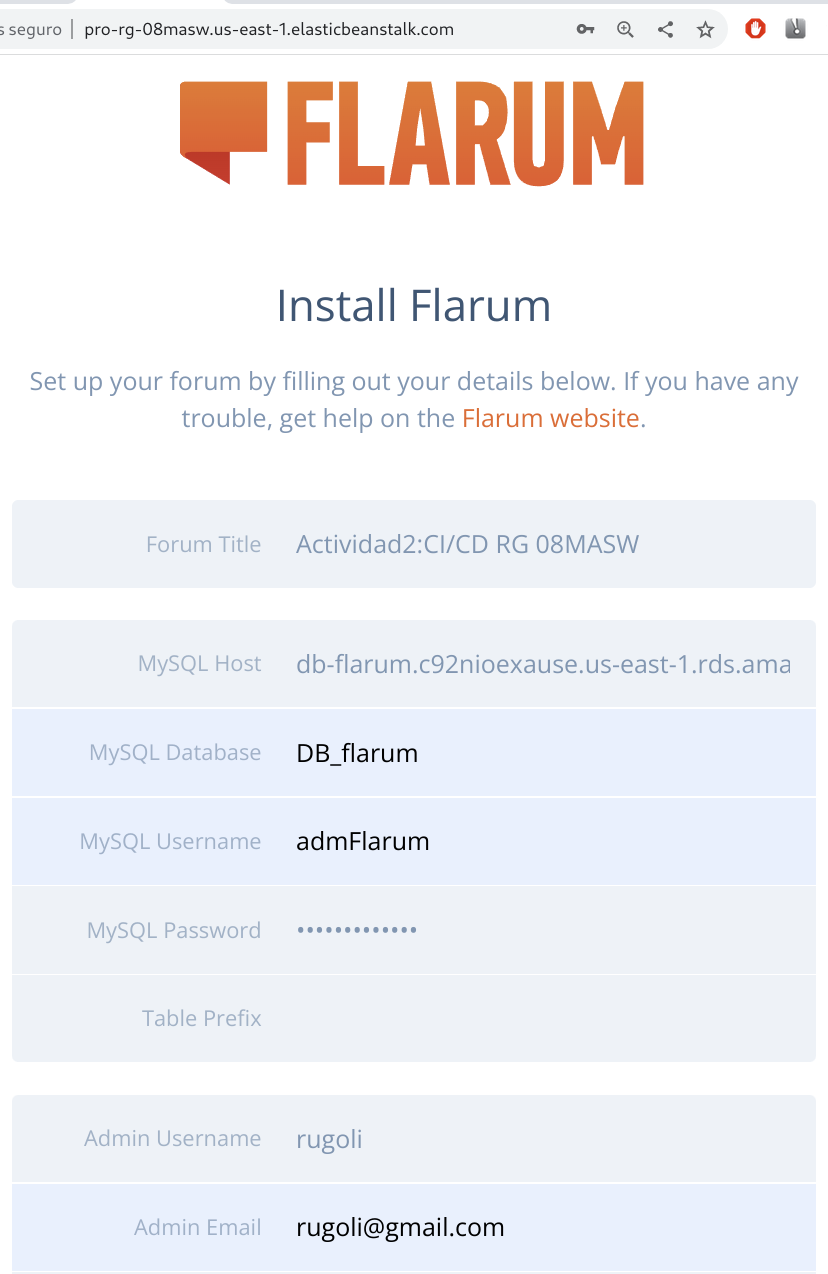
\includegraphics[frame,width=0.63\linewidth]{img/flarum-2.png}
\end{center}

\begin{center}
    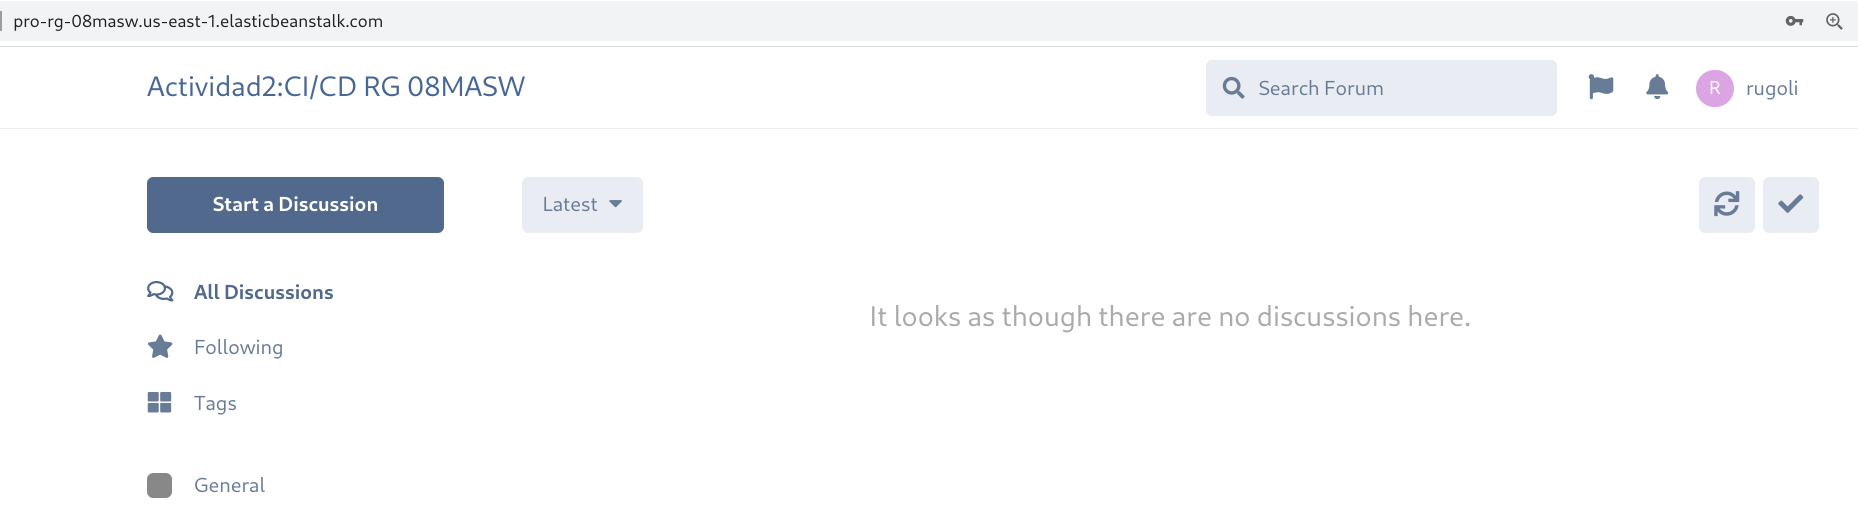
\includegraphics[frame,width=\linewidth]{img/flarum-3.png}
\end{center}


\begin{mycode}{Crear instancia RDS mediante CLI}{console}{}
ddd_v1_w_Hox_1818884@runweb70100:~$
\end{mycode}




\chapter{Conclusiones}

Tal como se ha podido ver, l

\end{document}
